% Inicio del preámbulo

\documentclass[letterpaper,12pt]{article} %Modifica el tipo de documento y el tamaño de la letra.
\usepackage[utf8]{inputenc} %Formato UTF-8 para caracteres especiales.
\usepackage[shortlabels]{enumitem}
\usepackage[spanish,mexico]{babel} 
\usepackage{amsmath,amssymb,amsfonts,latexsym,cancel}
\usepackage{hyperref}
\usepackage{wrapfig}
\usepackage[rflt]{floatflt}
\usepackage[pdftex]{graphicx}
\usepackage{fancyhdr} %Paquete para el header y el formato de la portada. No sugiero borrarlo!
\usepackage{float}
\usepackage{longtable,multirow,booktabs}
\usepackage{cite}
\usepackage{wrapfig}
\usepackage[square,numbers]{natbib}
\usepackage{multicol}
\usepackage{caption}
\usepackage[]{sidecap}
\usepackage{adjustbox}
\usepackage{parskip}
\usepackage{enumitem}
\usepackage{tikz}
\usepackage{lipsum}
\usepackage[]{xcolor}
\usepackage{multirow}
\usepackage{colortbl}

%Fin de Préambulo
% Variables del documento
% Document Variables 
\newcommand{\myMateria}{CUADERNO DE INFORMES}
\newcommand{\myGrupo}{K}
\newcommand{\mySemester}{2023-10}
\newcommand{\MyReport}{Manejo de la Interfaz de Unity 3D}
\newcommand{\myUnidad}{I}
\newcommand{\myDate}{15 de mayo de 2023}
\newcommand{\myName}{Alex Diego Rosas Quispe}
\newcommand{\myTeacher}{Norman Patrick Harvey Arce}



%Inicio formato de Página. 

\textheight = 21cm %Medidas de la  página
\textwidth = 18cm  %Medidas de la página
\topmargin = -2cm  %Medidas de la página    
\oddsidemargin = -0.8cm %Medidas de la página
\pagestyle{fancy} %Diseño de la página

\fancyhf{}
\lhead{\myMateria}%%LeftHead
\chead{
\includegraphics[ height=1cm]{Imágenes/senati.png}}%%CenterHead
%\lfoot{USM}
\rhead{Unidad \myUnidad}%%RightHead

\setlength{\columnsep}{4mm}%Comandos para el formato de la página.
%\setlength{\parindent}{4em}%Sangría al comenzar un nuevo párrafo.
\setlength{\parindent}{0.5in}
%\setlength{\parindent}{4em}%Sangría al comenzar un nuevo párrafo.
\setlength{\parskip}{1em}%Distancia entre párrafos.
\renewcommand{\baselinestretch}{1.0}% Espacio entre línea y línea o interlineado.
\setlength{\headheight}{33pt}
\fancyfoot[C,CO]{\thepage} %Logo de LaTeX y pie de página.

%Fin formato de Página

%Aquí inicia el documento.

\begin{document}

    %LaTeX te hace el índice automáticamente conforme añades secciones en tu documento.
    \thispagestyle{empty}
			\begin{figure}[ht]
		   \minipage{0.7\textwidth}
				
\includegraphics[width=5cm]{Imágenes/senati.png}
				\label{escudoTecNM}
		   \endminipage
		   \minipage{\textwidth}
				%
\includegraphics[width=3cm]{Imágenes/SENATI.jpg}
				\label{EscudoITCJ}
			\endminipage
				%%\vspace{-1cm}
		\end{figure}
		
		\vspace{0.1cm}
		
		\begin{center}
		    {\scshape\LARGE \textbf{Servicio Nacional de Adiestramiento en Trabajo Industrial} \par}
			{\scshape\Large Facultad de Tecnologías de la Información \par}
			{\scshape\large Escuela de Diseño y Desarrollo de Videojuegos y Realidad Aumentada \par}
            \vspace{0.75cm}
             {\Large \textbf{\myMateria}}

			% Restauramos el interlineado:
			\begin{center}
			
			
			%{\Large Grupo:\myGrupo}
			\vspace{0.75cm}
				
			{\LARGE\bfseries \MyReport\\Unidad \myUnidad\par}
            \vspace{0.75cm}
            
		{\scshape\Large Fecha de entrega: \myDate\par}	
        \vspace{0.75cm}
	    \LARGE	{ \textbf{Profesor:}}\\
        \large		{ \myTeacher}
        
		\vspace{0.5cm}	
		
		\LARGE	{ \textbf{Alumno:}}
        
        \normalsize	 {\myName}

%% \it es letra itálica
				\vspace{1.25cm}
				\vspace{0.9cm}
				
			\end{center}
	
		\end{center}

    \newpage
%Inicio parte opcional. Esta parte la puedes quitar si deseas, es por si te piden formatos para
%evidencias de certificación de los laboratorios con números de cuenta o te piden abstracts en tus %trabajos.

% \title{\myMateria \\\textbf{\MyReport} \\ } 
\author{ \normalsize{\texttt{\myName}} }
% \date{\myDate}
% \maketitle
\thispagestyle{fancy}


%Fin parte opcional
\begin{table}[t]
  \begin{center}
    \begin{tabular}{ c  c  c  c  c  c  }
      \multicolumn{5}{c}{}& \multicolumn{1}{r}{\textbf{DIRECCIÓN ZONAL}} \\    
      \multicolumn{6}{c}{} \\
      \multicolumn{5}{c}{}& \multicolumn{1}{r}{ Arequipa - Puno}\\
      \multicolumn{6}{c}{} \\
      \multicolumn{2}{c}{} & \multicolumn{2}{c}{} & \multicolumn{2}{c}{\textbf{FORMACIÓN PROFESIONAL}}\\
      \multicolumn{6}{c}{} \\ 
      \multicolumn{6}{c}{} \\
      \multicolumn{1}{l}{CFP/UCP/ESCUELA:} & \multicolumn{5}{c}{CFP Arequipa/UPC Arequipa /Tecnologías de la Información} \\ 
      \multicolumn{6}{c}{} \\
      \multicolumn{1}{l}{ESTUDIANTE:} & \multicolumn{5}{l}{Alex Diego Rosas Quispe} \\ 
      \multicolumn{6}{c}{} \\
      \multicolumn{1}{l}{ID:} & \multicolumn{5}{l}{001363405} \\
      \multicolumn{6}{c}{} \\
      \multicolumn{1}{l}{BLOQUE:} & \multicolumn{5}{l}{202310-CNIU-108-ACT-NRC-91705} \\
      \multicolumn{6}{c}{} \\
      \multicolumn{1}{l}{CARRERA:} & \multicolumn{5}{l}{Diseño y Desarrollo de Videojuegos y Realidad Aumentada} \\
      \multicolumn{6}{c}{} \\
      \multicolumn{1}{l}{INSTRUCTOR:} & \multicolumn{5}{l}{Norman Patrick Harvey Arce} \\ 
      \multicolumn{6}{c}{} \\
      \multicolumn{1}{l}{SEMESTRE:} & \multicolumn{5} {l} {V semestre DEL: 17-04-2023 AL: 31-07-2023} \\
    \end{tabular} 
  \end{center}
\end{table}

\section*{\centering\textbf{INSTRUCCIONES PARA EL USO DEL CUADERNO DE INFORMES}}
\vspace{1cm}
\section{\normalsize{ PRESENTACIÓN.}}

El cuaderno de informes es un documento de autocontrol, en el cual el estudiante,
registra diariamente, durante la semana, las tareas, operaciones que ejecuta en su
aprendisaje, es un medio para desarrollar la Competencia de Redactar Informes. 

\section{\normalsize{INSTRUCCIONES PARA EL USO DEL CUADERNO DE INFORMES}}
\begin{itemize}
\item {En la hoja de informe semanal, el estudiante registrará los trabajos
que ejecuta, indicando el tiempo correspondiente. El día de asistencia 
registraá los contenidos que desarrolla. Al término de la semana totalizará
las horas.\\
De las tareas ejecutadas durante la semana, el ESTUDIANTE seleccionará la 
tarea más significativa y él hará una descripción del proceso de ejecución 
con esquemas, diagramas y dibujos correspondientes que aclaren dico proceso.}

\item {Semanalmente, el instructor revisará y calificará el Cuaderno de Informes
haciendo las observaciones y recomendaciones que considere convenientes, en los 
aspectos relacionados a la elaboracion de un Informe Técnico (letra normalizada,
dibujo técnico, descripción de la tarea y su procedimiento, normas técnicas,
seguridad, etc.)}

\item {Escala de calificación vigesimal}
\end {itemize}

\vspace{2cm}

\begin{table}[!ht]
  \centering
  \begin{tabular}{| c | c | c |}
    \hline
    \rowcolor{gray!30}
    \textbf{CUANTITATIVA} & \textbf{CUALITATIVA} & \textbf{CONDICIÓN} \\ \hline
    $16.8-20.0$ & Excelente & \multirow{3}{*}{Aprobado} \\ \cline{1-2}
    $13.7-16.7$ & Bueno &  \\ \cline{1-2}
    $10.5-13.6$ & Aceptable &  \\ \hline
    $00-10.4$   & Deficiente & Desaprobado \\ \hline
  \end{tabular}
  \caption{Cuadro de calificaciones}
  \label{tab:calificaciones}
\end{table}


\section*{\centering{\large{INFORME SEMANAL}}}

V SEMESTRE SEMANA N° 1

\begin{table}[!ht]
  \begin{flushright}
    \begin{tabular}{| c | c | c | c |}
      \hline
      \rowcolor{gray!50}
              & Día & Mes & Año \\ \hline
      Del     &   17  &   05  & 2023    \\ \hline
      Al      &  22   &   05  &  2023   \\ \hline
    \end{tabular} 
  \end{flushright}
\end{table}

\vspace{1cm}
\begin{table}[!ht]
  \centering
  \begin{tabular}{| p{3cm} | p{10cm} | c |}
    \hline
    \rowcolor{gray!50}
    \textbf{DÍA} & \textbf{TAREAS EFECTUADAS} & \textbf{HORAS} \\ \hline
    LUNES &Historia de los videojuegos, introducción al desarrollo de videojuegos, motores de videojuegos ventajas y desventajas. & \large4h:00min\\ \hline
    MARTES &Importación de modelos 3D manejo de texturas y materiales. & \large1h:30min \\ \hline
    MIÉRCOLES & & \\ \hline 
    JUEVES & & \\ \hline
    VIERNES & & \\ \hline
    SABADO & Unity modelos de negocio, portfolio , ventajas y desventajas. Unreal, Godot, GameMaker.  & \large4h:45min\\ \hline
  & \textbf{TOTAL}& \large10h:15min\\ \hline
  \end{tabular}
  \caption{Cuadro de informe semanal}
  \label{tab:informe-semanal}
\end{table}


\section*{\centering\large{INFORME DE TAREA MÁS SIGNIFICATIVA}}

\textbf{Tarea: Motores de Videojuegos}\\ 

\textbf{Descripción del proceso:}\\ 

Un motor de videojuegos es un software específicamente para facilitar el desarrollo y la creación de videojuegos. Es una colección de herramientas, bibliotecas y sistemas que permiten a los desarrolladores de juegos crear, diseñar y programar juegos de manera mas eficiente.

El motor de un videojuego proporciona una serie de funcionalidades básicas que son necesarias para la creación de juegos, como la representación gráfica en 2D o 3D, la gestión del sonido, la física del juego, la inteligencia artificial, el manejo de colisiones, la animación, la gestión de recursos y otros aspectos técnicos. También suele incluir herramientas de desarrollo, como un editor de niveles, un sistema de scripting o un depurador, que ayudan a los desarrolladores a crear contenido y a depurar sus juegos.

Los motores de videojuegos permiten a los desarrolladores centrarse en la creación de contenido y la jugabilidad, en lugar de tener que preocuparse por programar desde cero todas las funcionalidades básicas de un juego. Al utilizar un motor de videojuegos, los desarrolladores pueden ahorrar tiempo y esfuerzo, ya que muchas tareas técnicas complejas están predefinidas y listas para usar.

Existen diferentes motores de videojuegos disponibles en la industria, como Unity, Unreal Engine, CryEngine y Godot, entre otros. Cada motor tiene sus propias características, fortalezas y limitaciones, y los desarrolladores pueden elegir el que mejor se adapte a sus necesidades y habilidades.

\textbf{VENTAJAS}

\begin{itemize}
	\item \textbf{Ahorro de tiempo:} proporcionan una base sólida y una serie de herramientas preconstruidas.
	
	\item \textbf{Flexibilidad:} permiten personalizar y ajustar los aspectos técnicos del juego según necesidades específicas.
	
	\item\textbf{Multiplataforma:} permiten crear juegos para distintas plataformas.
	
	\item\textbf{Comunidad:} tienen una gran comunidad de desarrolladores que comparten recursos, consejos y soluciones a problemas.
\end{itemize}
\newpage
\textbf{DESVENTAJAS}

\begin{itemize}
	\item \textbf{Costo:} algunos motores pueden ser bastante costoso, especialmente para pequeños estudios o independientes.
	
	\item \textbf{Limitaciones creativas:} pueden proporcionar una estructura base para el desarrollo del juego, pero también pueden limitar la creatividad y la libertad del desarrollador.
	
	\item \textbf{Curva de aprendizaje:} algunos motores pueden requerir conocimientos avanzados de programación y habilidades técnicas.
	
	\item \textbf{Dependencia del motor:} pueden hacer que el desarrollador sea dependiente de ese motor especifico por sus características.
\end{itemize}

\begin{figure}[!ht]
	\centering
	
\includegraphics[scale=0.7]{Imágenes/motor.png}
\end{figure}
\newpage
\subsection{Importación de modelos a Unity}

Para importar un modelo a Unity, sigue los siguientes pasos:

\begin{enumerate}
	\item Preparación del modelo: Antes de importar el modelo a Unity, asegúrate de que el modelo esté en un formato compatible. Unity admite varios formatos de modelos 3D, como FBX, OBJ y Collada (DAE). Si tu modelo no está en uno de estos formatos, deberás convertirlo usando herramientas como Blender u otros software de modelado 3D.
	
	\item Creación de una carpeta de recursos: En el proyecto de Unity, crea una carpeta en la que puedas almacenar los recursos del modelo. Por ejemplo, puedes crear una carpeta llamada "Modelos".
	
	\item Importación del modelo: Arrastra y suelta el archivo del modelo en la carpeta de recursos que creaste. Unity comenzará a importar automáticamente el modelo y sus texturas asociadas si las hay. Puedes ver el progreso de la importación en la barra de progreso de Unity.
	
	\item Ajuste de las propiedades del modelo: Una vez que el modelo esté importado, puedes ajustar sus propiedades en el inspector de Unity. Esto incluye la escala, la posición, la rotación y otros ajustes específicos del modelo.
	
	\item Uso del modelo en la escena: Ahora puedes utilizar el modelo importado en tu escena. Arrastra y suelta el modelo desde la carpeta de recursos a la jerarquía de objetos de la escena o colócalo mediante scripts en tiempo de ejecución.
\end{enumerate}
\section*{\centering\large{HACER ESQUEMA, DIBUJO O DIAGRAMA}}

\begin{figure}[!ht]
	\centering
	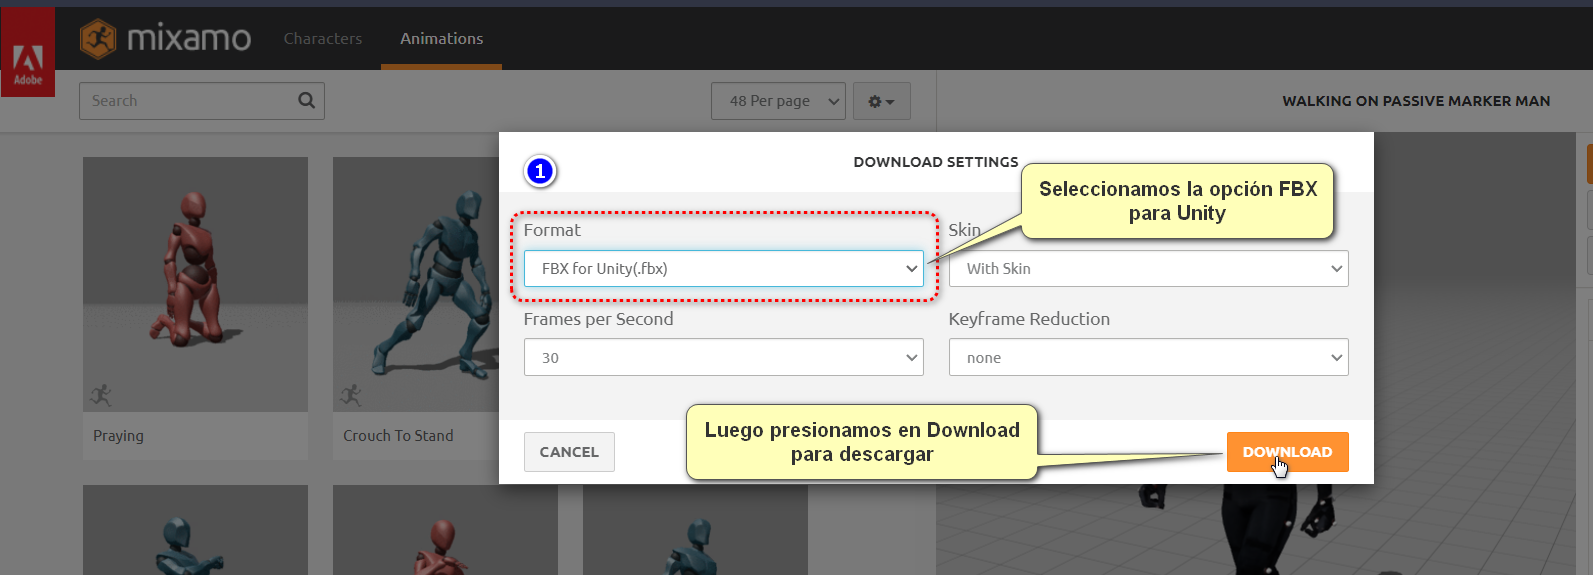
\includegraphics[scale=0.5]{Imágenes/paso1.png}
	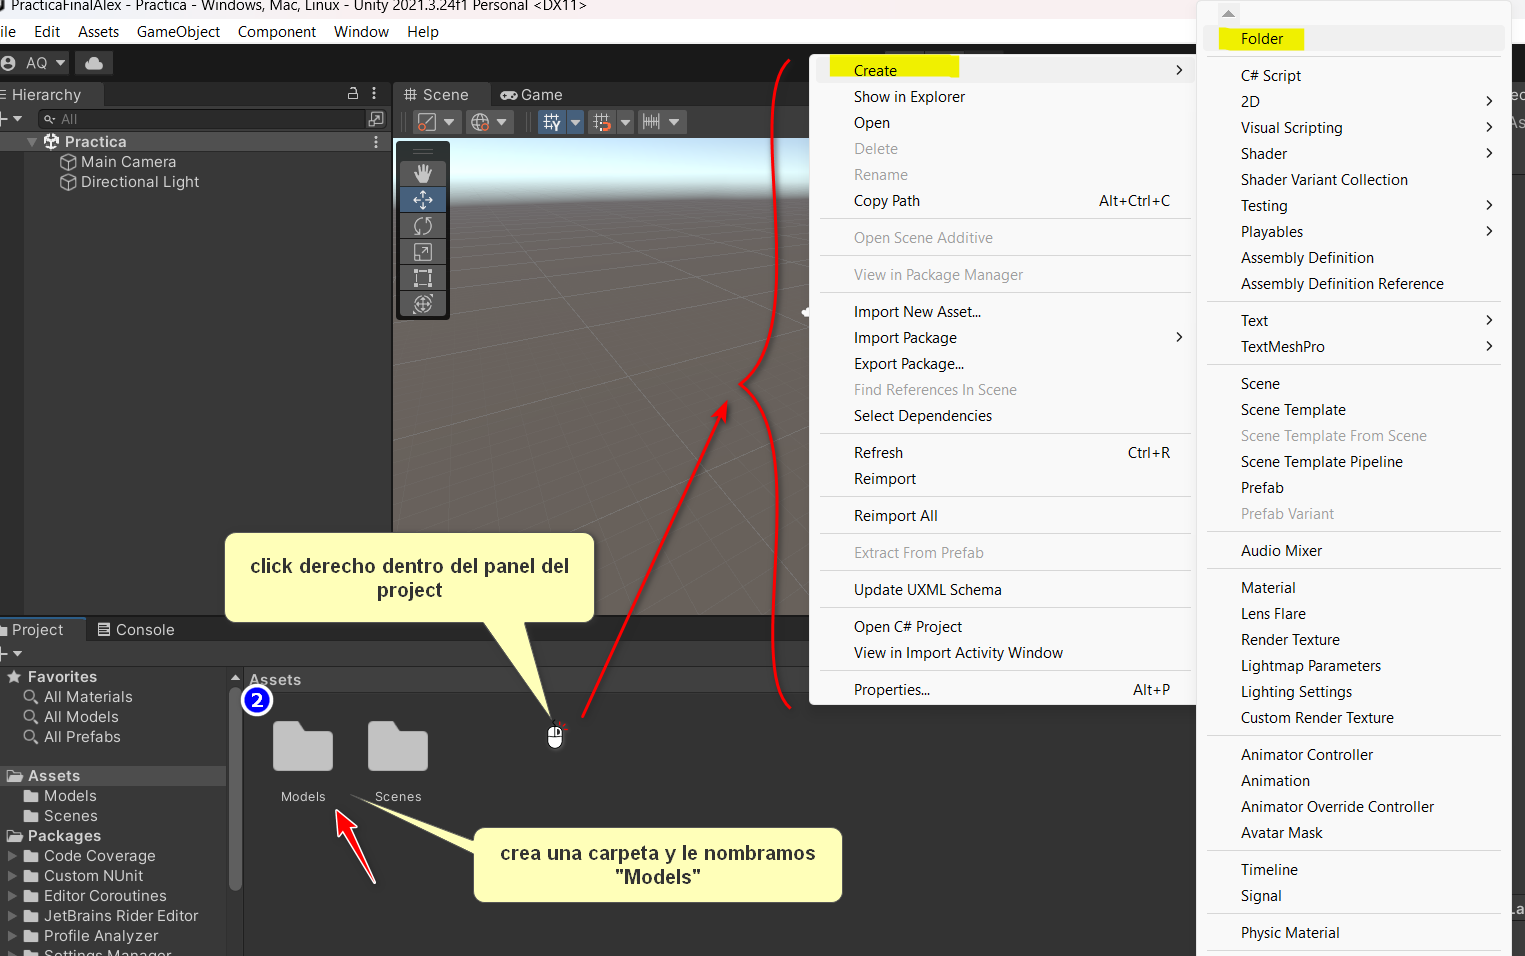
\includegraphics[scale=0.5]{Imágenes/paso2.png}
\end{figure}
\begin{figure}[!ht]
	\centering
	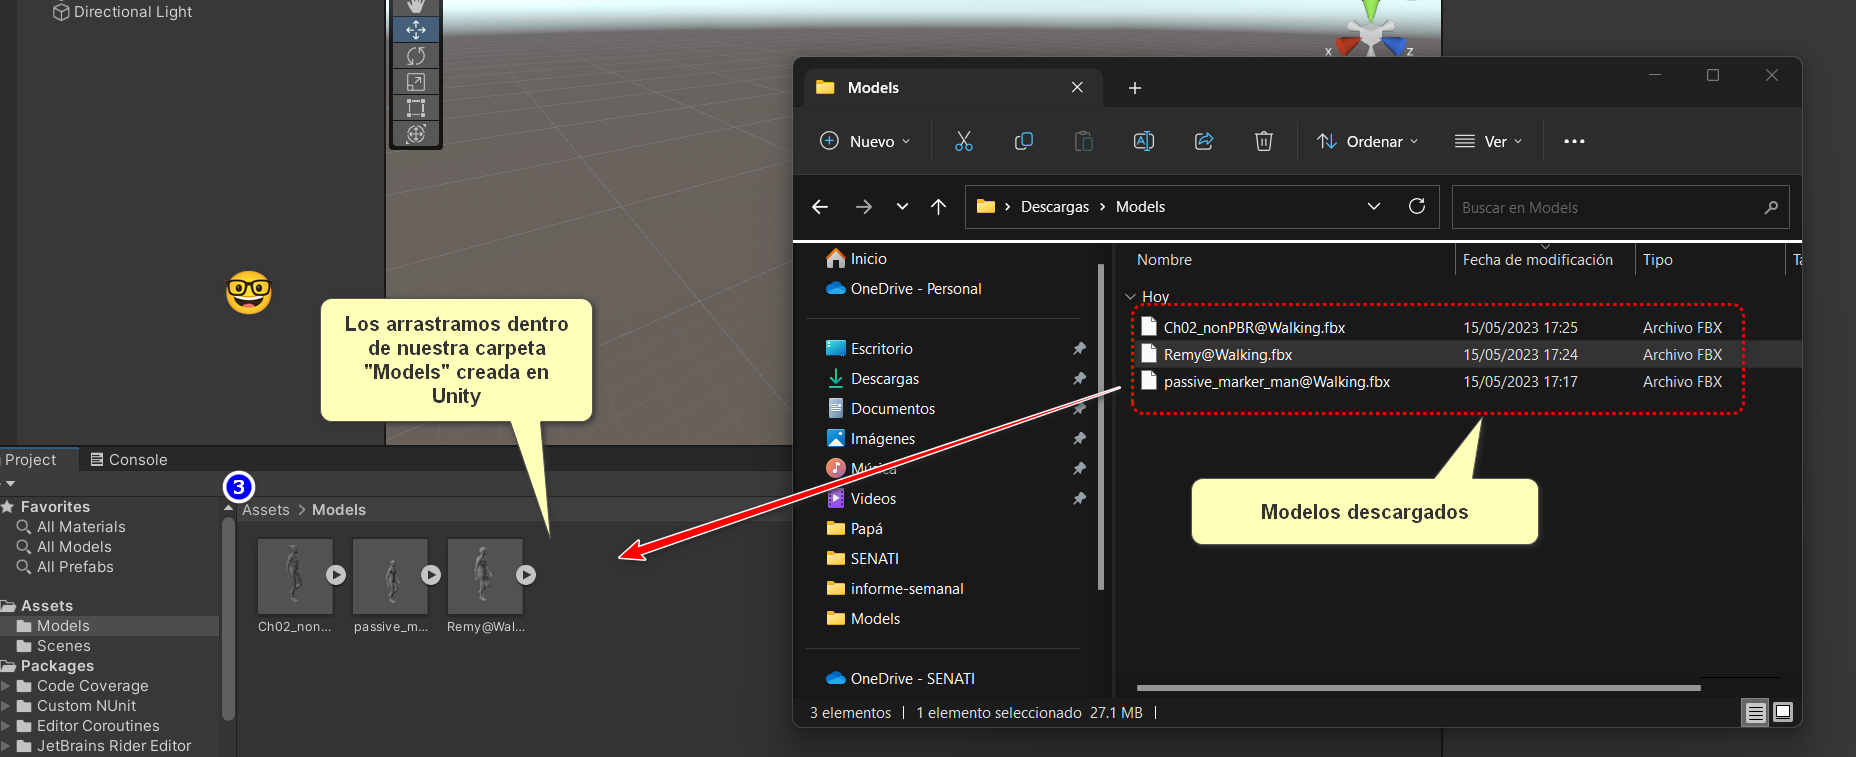
\includegraphics[scale=0.5]{Imágenes/paso3.png}
	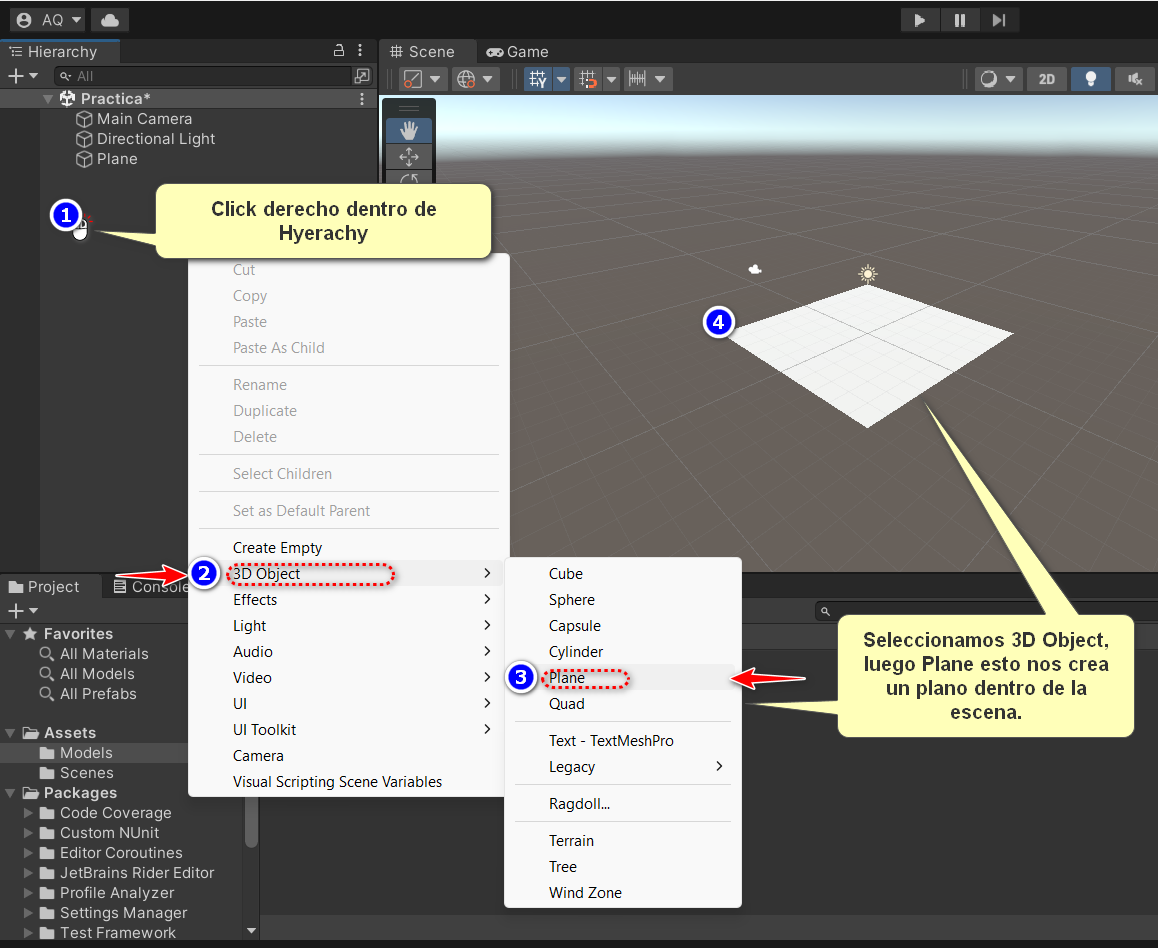
\includegraphics[scale=0.6]{Imágenes/paso4.png}
\end{figure}
\begin{figure}[!ht]
	\centering
	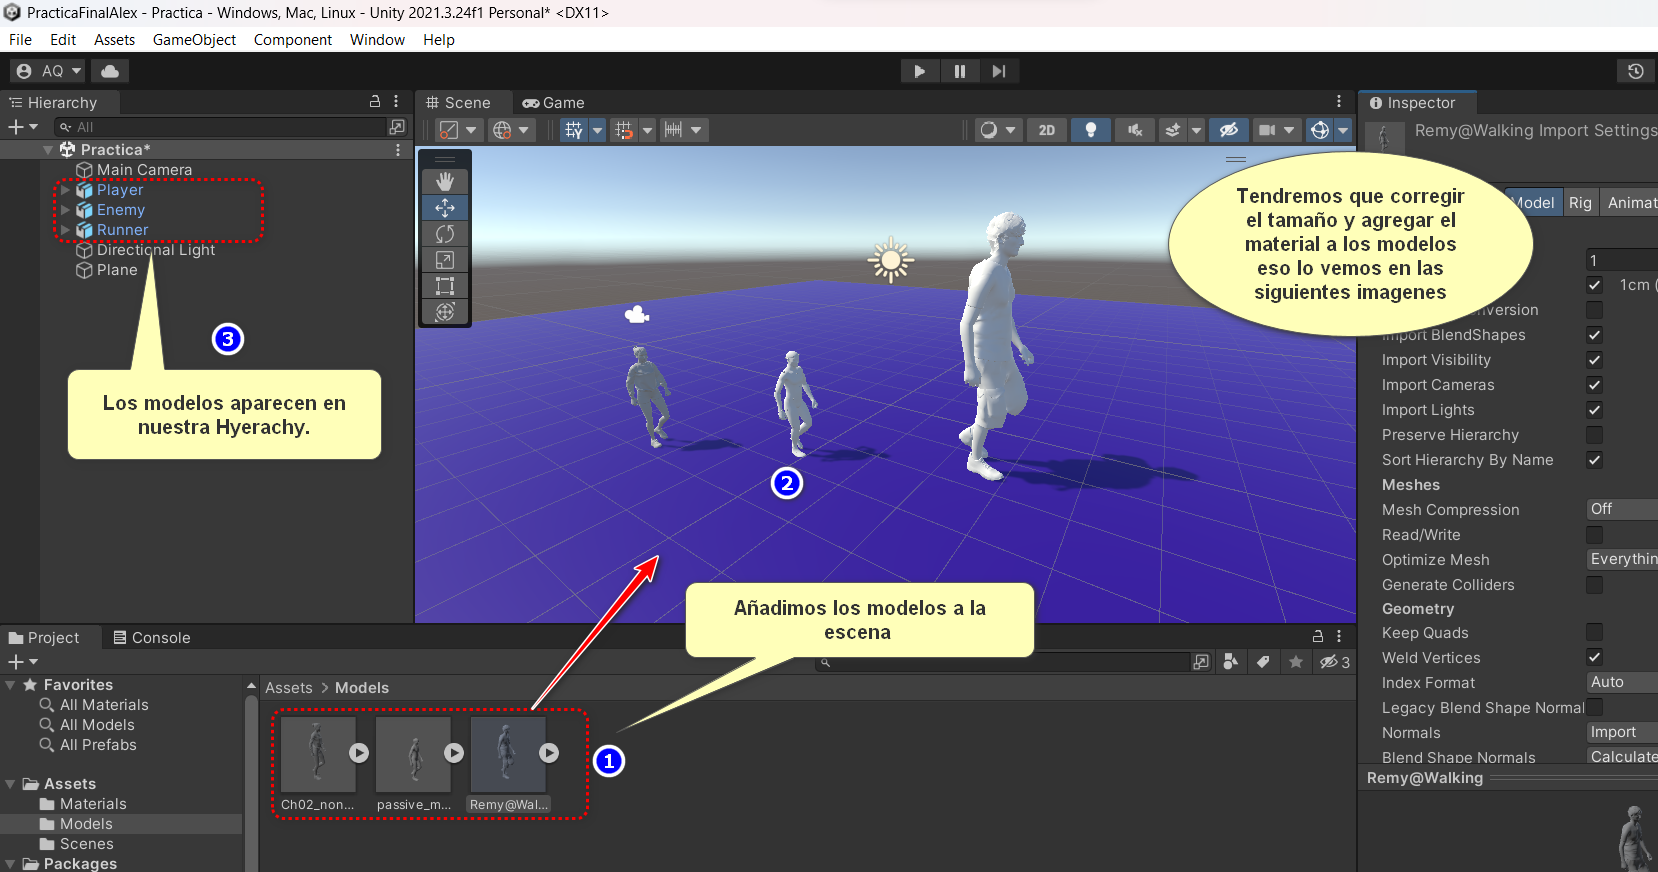
\includegraphics[scale=0.5]{Imágenes/paso5.png}
	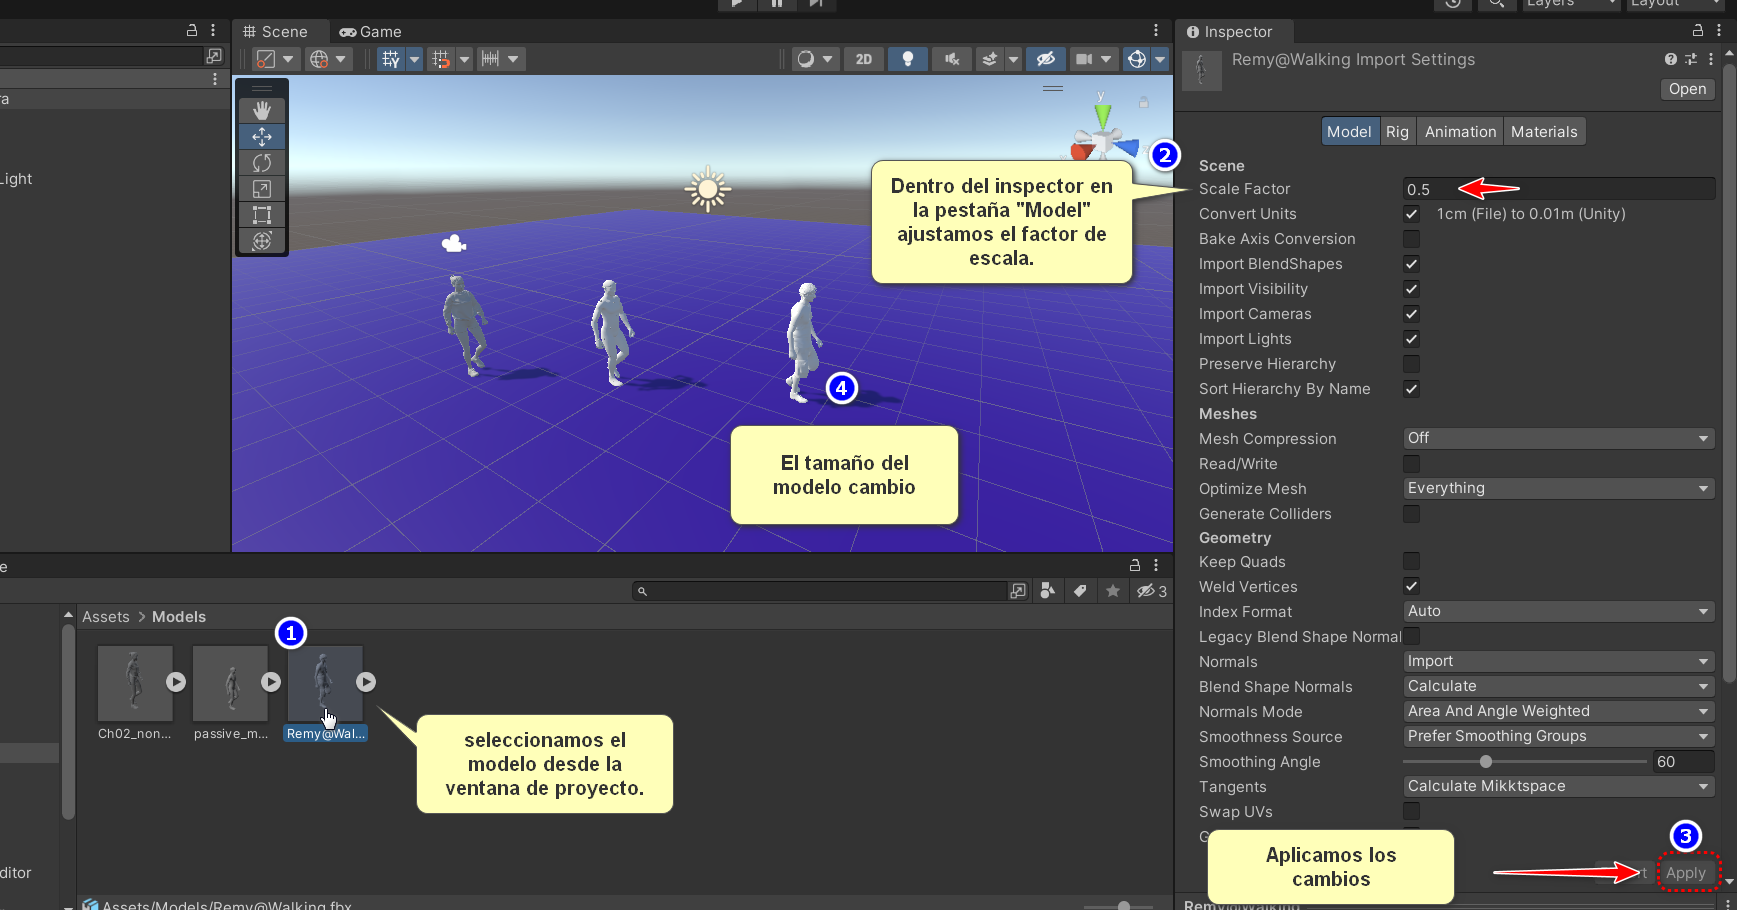
\includegraphics[scale=0.5]{Imágenes/paso6.png}
\end{figure}
\begin{figure}[!ht]
	\centering
	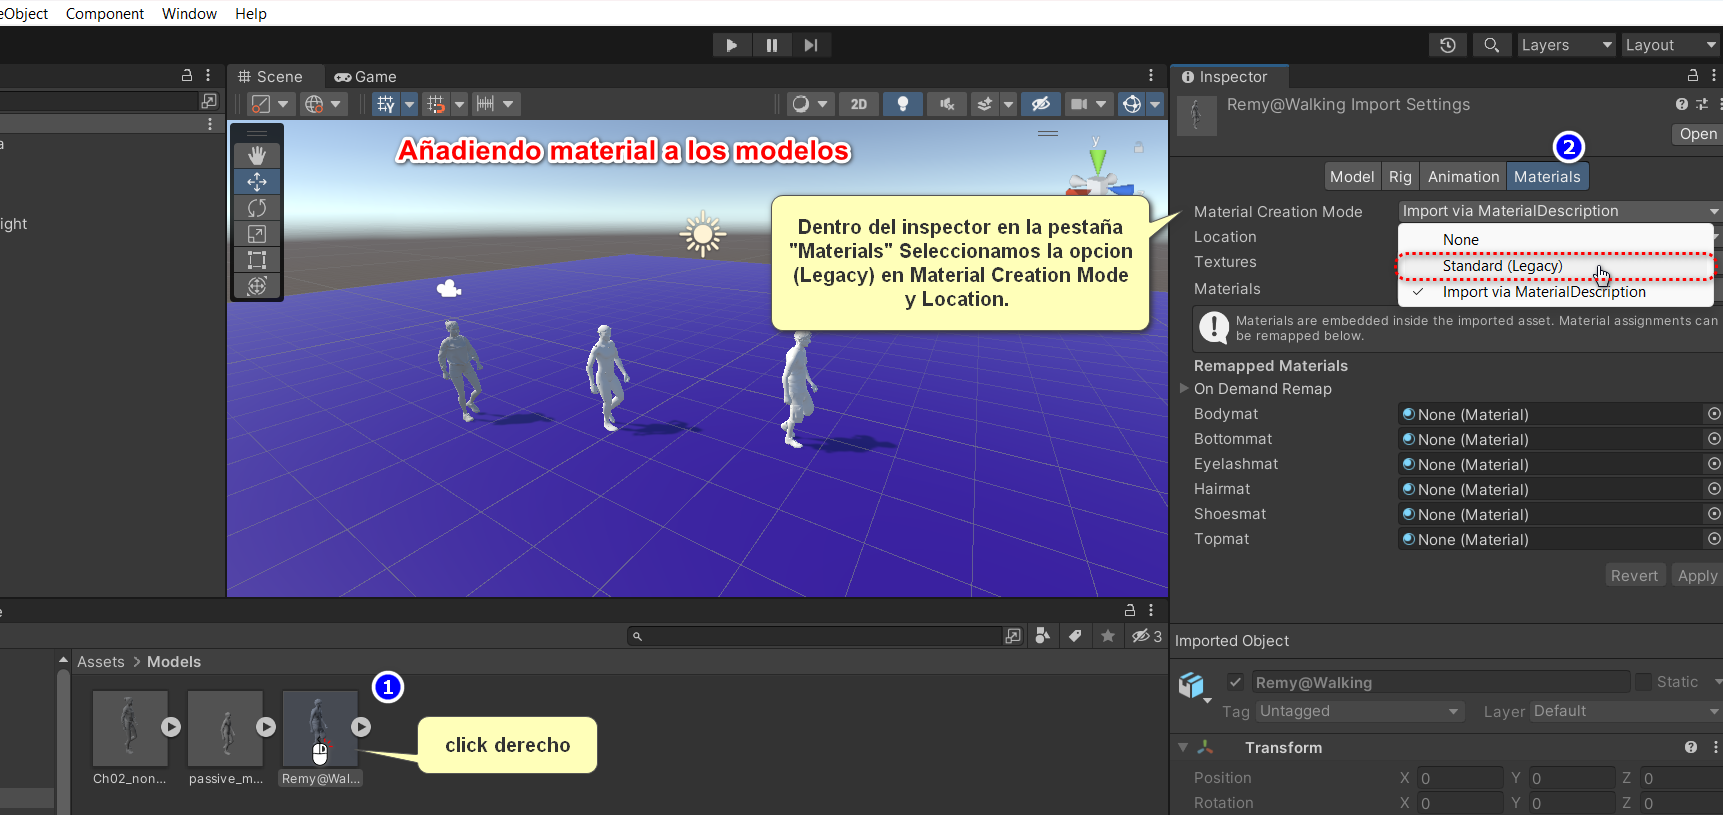
\includegraphics[scale=0.5]{Imágenes/paso7.png}
	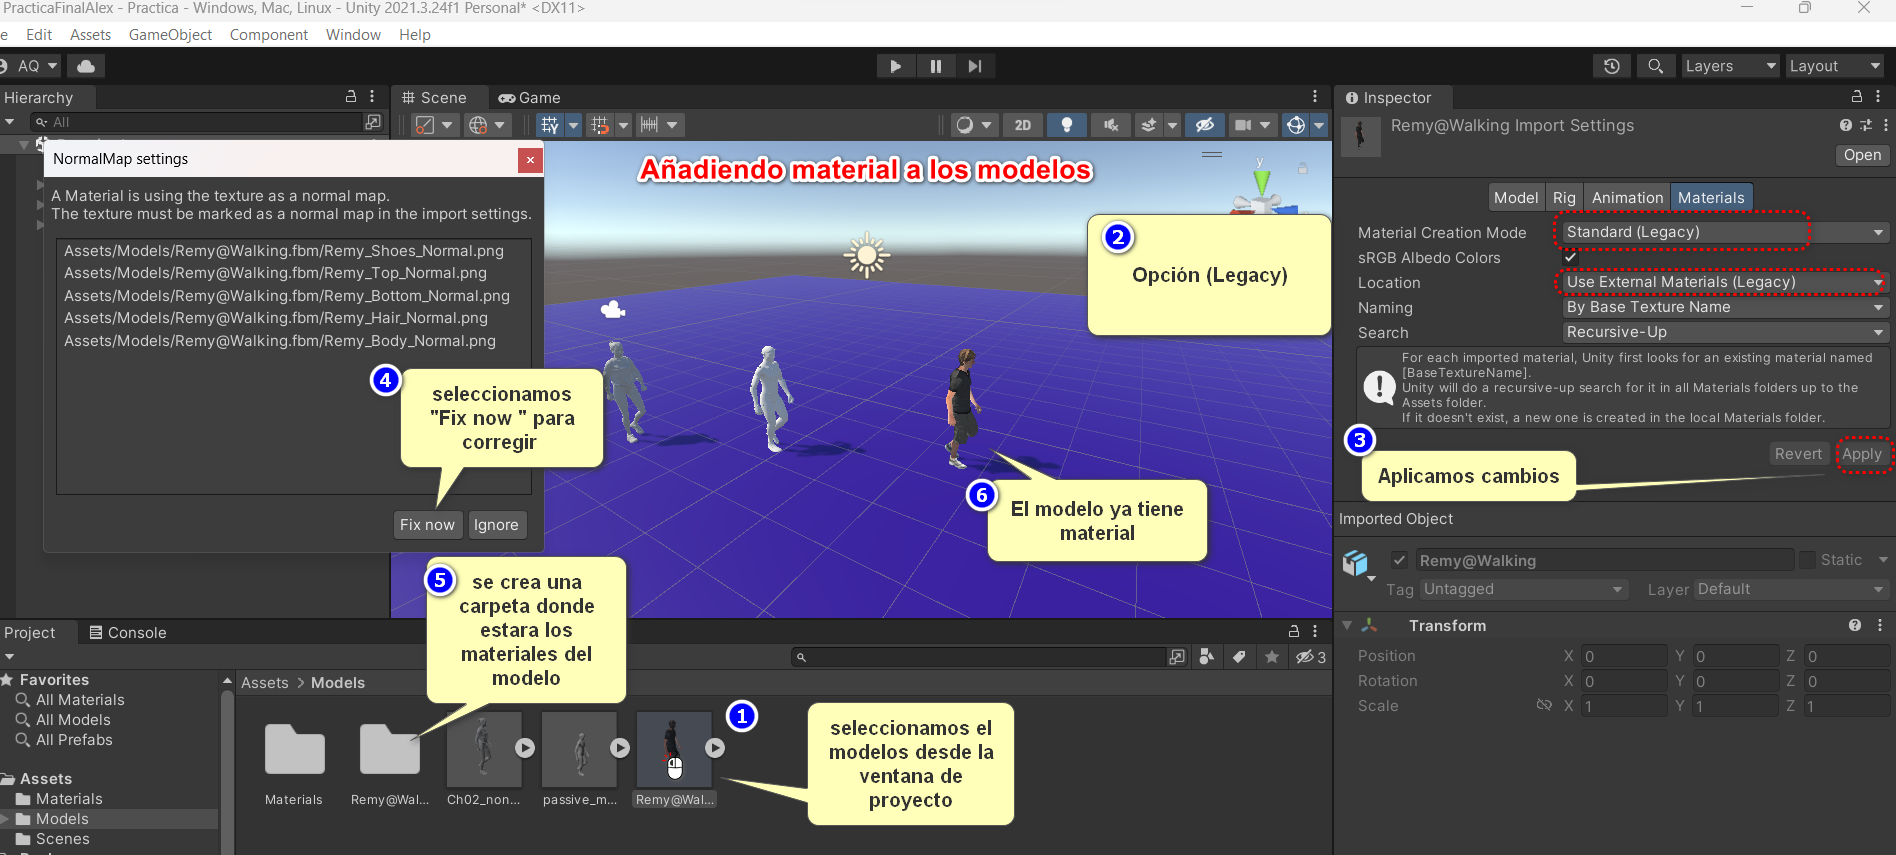
\includegraphics[scale=0.45]{Imágenes/paso8.png}
\end{figure}




\begin{center}
	\framebox{\fbox{\begin{minipage}{\dimexpr\linewidth-2\fboxsep-2\fboxrule}
				\centering{\textbf{EVALUACIÓN DEL INFORME DE TRABAJO SEMANAL}}
				\vspace{0.5cm}
				\begin{flushright}
					\begin{tabular}{c|p{1cm}|}
						\cline{2-2}
						\Large\textbf{Nota} & \\
						\cline{2-2}
					\end{tabular}
				\end{flushright}
	\end{minipage}}}
\end{center}

\begin{table}[!ht]
	\begin{center}
		\begin{tabular}{| p{9cm} | p{8.3cm} |}
			\hline
			\multicolumn{2}{|c|}{\textbf{OBSERVACIONES Y RECOMENDACIONES}}\\ \hline
			\multicolumn{2}{|p{17cm}|}{DEL INSTRUCTOR: } \\ \hline
			\multicolumn{2}{|p{17cm}|}{} \\ \hline
			\multicolumn{2}{|p{17cm}|}{} \\ \hline 
			\multicolumn{2}{|p{17cm}|}{} \\ \hline 
			\multicolumn{2}{|p{17cm}|}{} \\ \hline
			\multicolumn{2}{|p{17cm}|}{} \\ \hline 
			\multicolumn{2}{|p{17cm}|}{} \\ \hline 
			\multicolumn{2}{|p{17cm}|}{} \\ \hline
			FIRMA DEL ESTUDIANTE & FIRMA DEL INSTRUCTOR \\ \hline
			& \\  &\\ & \\ & \\ & \\ \hline
		\end{tabular}
	\end{center}
\end{table}
\begin{figure}[p]
\centering

\includegraphics[scale=0.3]{Imágenes/senati.png}
\end{figure}



% \nocite{*}
% \bibliographystyle{apalike}
% \bibliography{Libros.bib}


%Pequeño disclaimer por si usas fotos con derechos de autor que sacaste de Internet. Nunca está de más. 
%\centering \small Los créditos de las fotografías pertenecen a sus respectivos autores.
%
% \centering\vspace*{\fill} 
\end{document}

 %Fin del documento.
